\subsection{\rqone}
\label{sec:results:rq1}
\subsubsection{Motivation}
In this research question, we look to see whether there are any common characteristics of packages that release in-range breaking updates, and what types of updates end up breaking a client's build. In-range breaking updates are problematic for clients and finding common features of these updates is the first step in attempting to eliminate them.

\subsubsection{Approach}
We first wanted to see how the in-range breaking updates were distributed across different update types. Recall that semantic versioning splits updates into three primary categories: \textit{patch}, \textit{minor} and \textit{major} updates. On the breaking build issue reports, we extract the version the dependency was being updated from and the version the dependency was being updated to in order to determine whether the release was a major, minor, or patch update. We also want to compare how the number of in-range breaking updates by type compare to how often these update types are being released, as well as how often these update types are actually accepted by client version specifications.
\par
To determine what proportion each update type has of all releases, we examine all of the versions each of the dependency to determine how many patch, minor, and major updates the package has released. We determined what types of updates clients accept from providers by extracting each client's development and run-time dependency version specifications, and determining the type of updates they accept based on the rules outlined in Table \ref{tab:semver}.
\par
Another factor we investigate was whether the release frequency of provider packages tends to have any affect on how often they release in-range updates that break their clients. We tally the number of in-range updates each provider has that broke their client's, and compare the distributions across the total number of releases that package has, as well as the frequency at which that package releases new versions.

\subsubsection{Results}
We were able to extract the version ranges of the breaking dependency being updates for 63.77\% of the issue reports. This is because Greenkeeper will bundle upgrades for the packages that have to be upgraded together, and if one of the updates in the bundle breaks the client's build, the issue report is opened for all of the updates in the bundle. We are not able to determine the specific breaking dependency in the bundle, and we therefore omit these issue reports from our analysis.
\par
We found that 65.15\%, 34.69\%, and 0.16\% of in-range breaking updates are patch, minor, and major updates, respectively. These results would suggest that package developers are not following the semantic versioning scheme, which states that only major updates should be used to signify a breaking change in the package. However, patch and minor updates occur much more frequently than major updates. We found that 64.37\%, 28.25\%, and 7.37\% of package releases were patch, minor and major updates, respectively. This explains to some degree why the number of in-range breaking updates that are patch and minor updates is larger than major updates, since patch and minor updates occur more frequently then major updates.
\par
Additionally, we found that major updates are far less likely to be accepted as in-range updates by clients. Recall that, in order for an update to be considered in-range, the client must specify the range of updates they are willing to accept. We found that 12.53\% of dependencies are pinned by clients, which means the provider will never be able to release an in-range update. Of the remaining dependencies, 3.74\%, 82.31\%, and 1.08\% are accepting patch, minor, and major updates, respectively, which would further reduce the number of major updates that are considered to be in-range for clients. These results are summarized in Figure \ref{fig:bar_stacked_breaks_releases_accepted_update_types}
\begin{figure}[h]
    \centering
    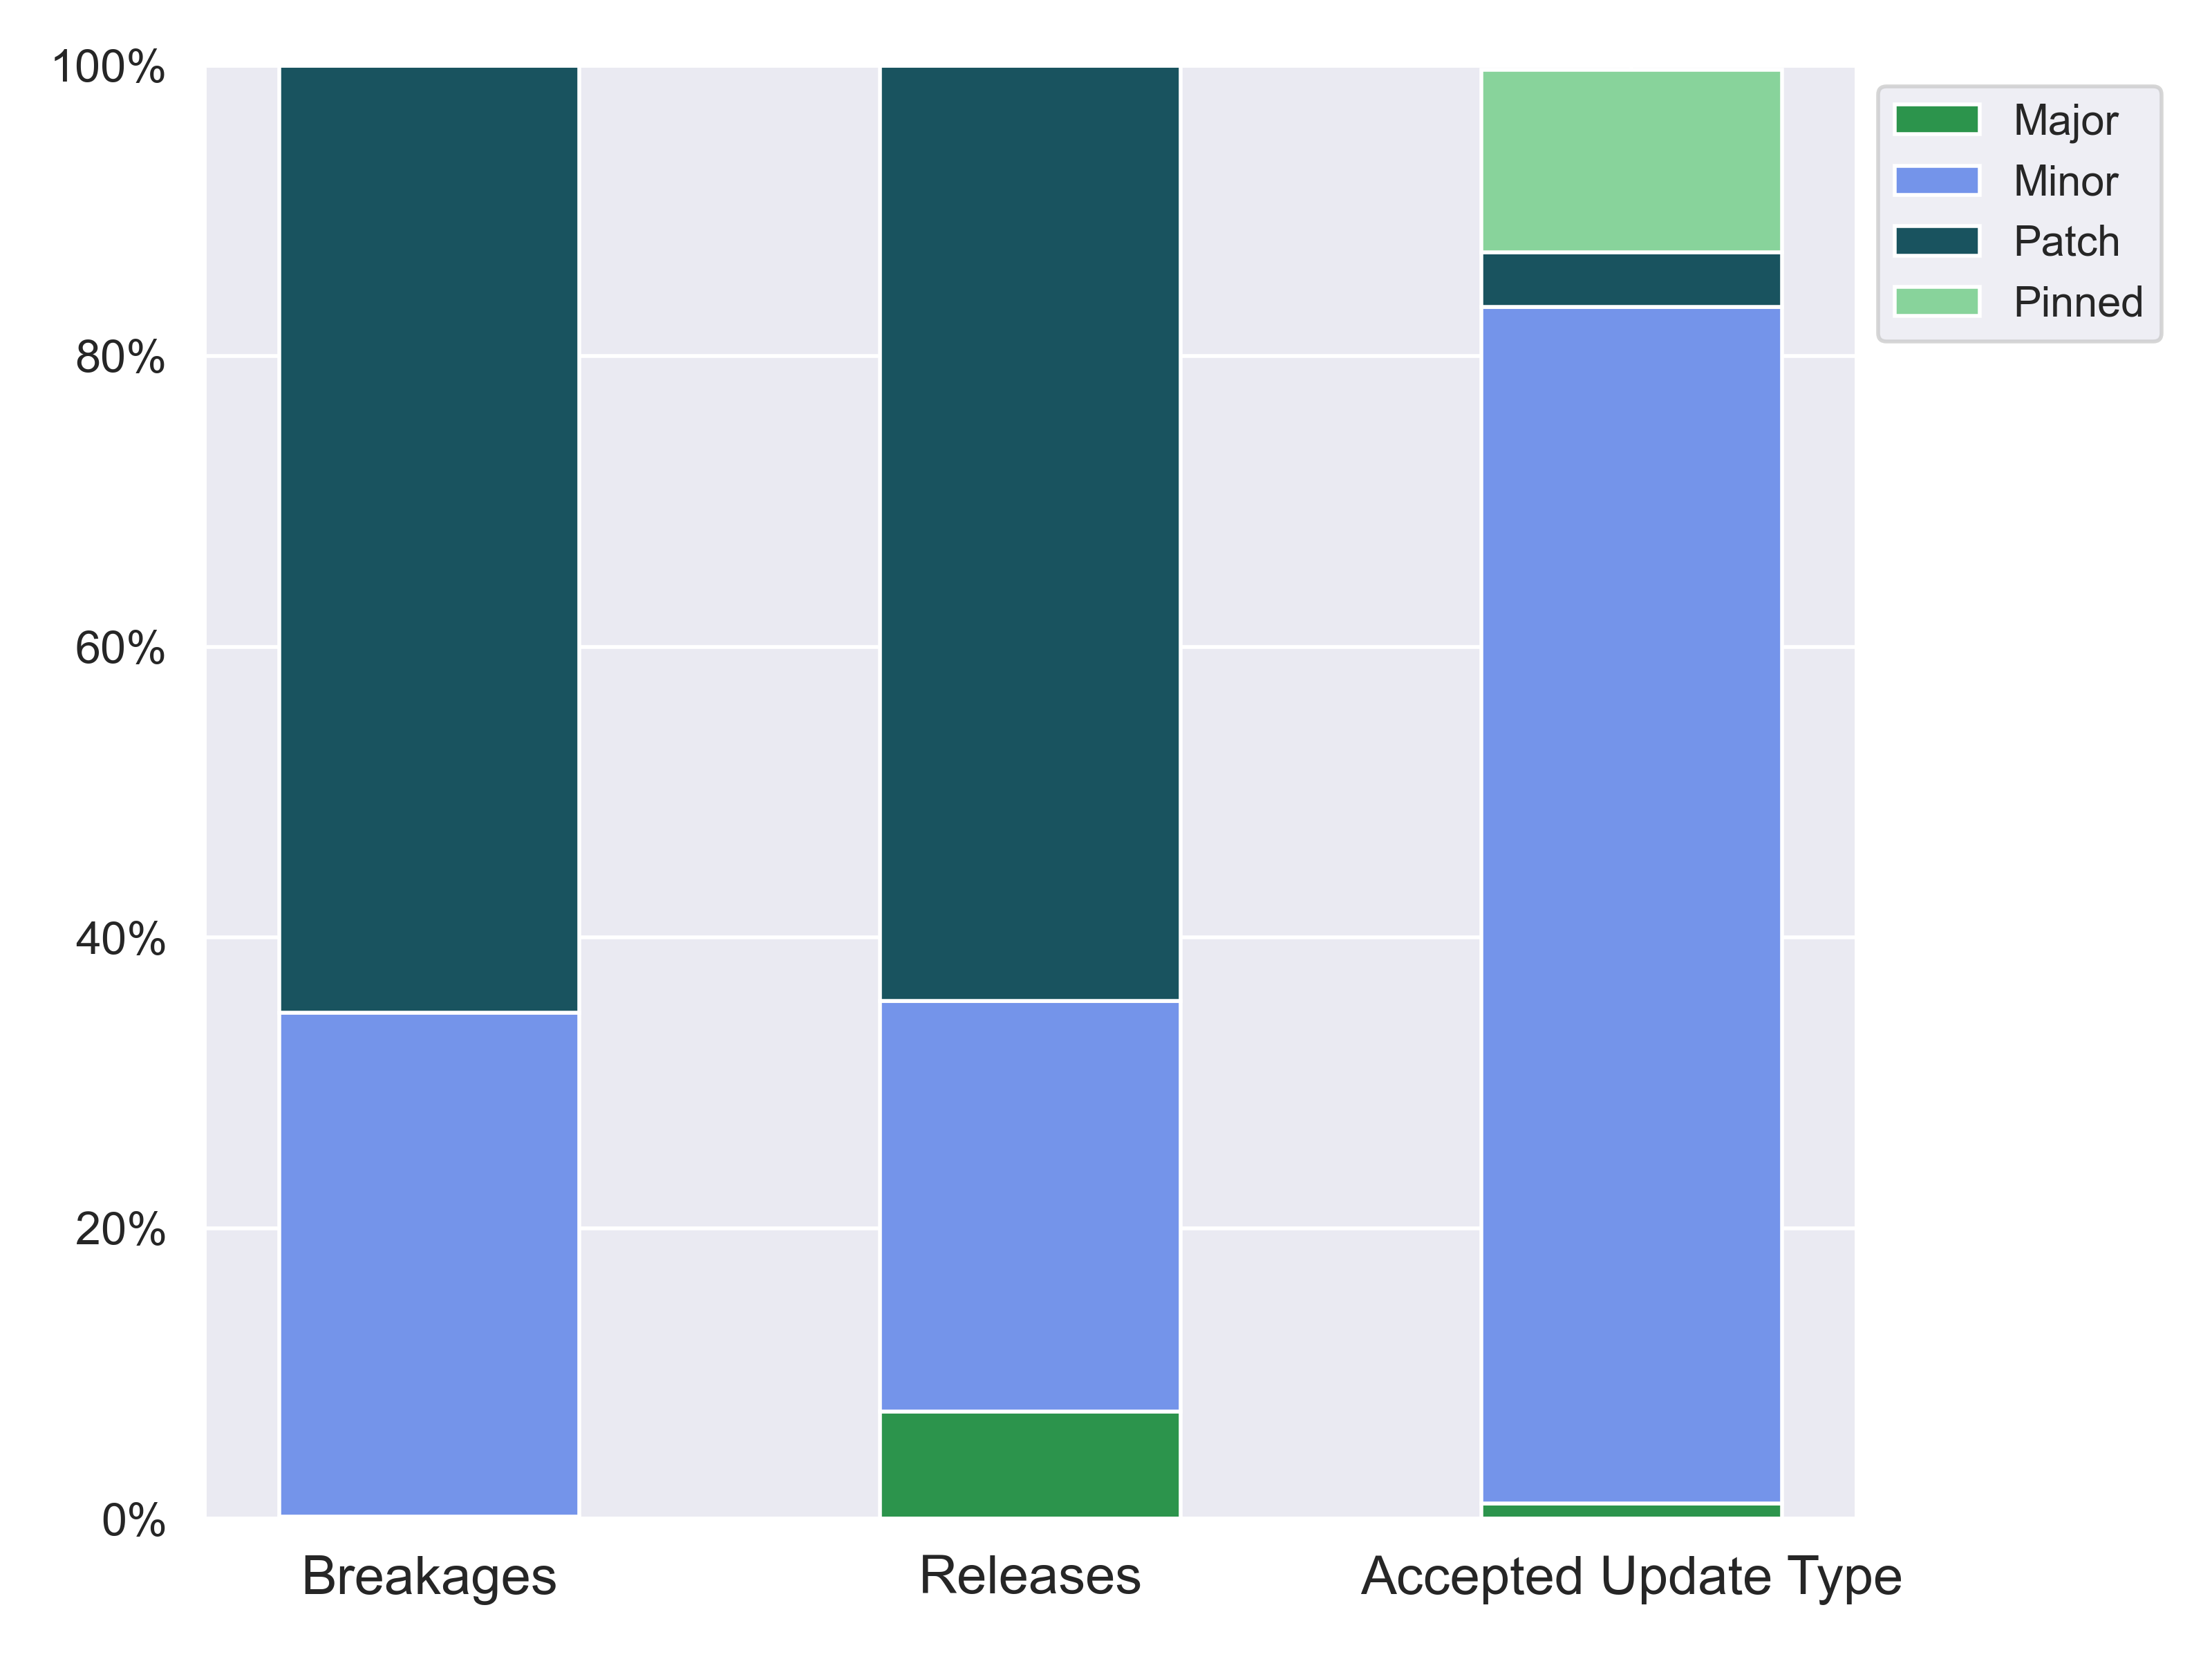
\includegraphics[width=\linewidth]{images/rq1_stacked.png}
    \caption{Distribution of update types for in-range breakages, package releases, and accepted update types}
    \label{fig:bar_stacked_breaks_releases_accepted_update_types}
\end{figure}
\par
In terms of how the release practices of packages affect how often they release in-range breaking updates, we found that the number of broken builds increases by 0.07 for every additional release a package makes. Intuitively, this result is expected. The more releases a package has, the more opportunities there are that a release will break a client's build. We also look at the distribution of build breakages caused by a provider against the frequency at which they release new versions. We found that the number of in-range breakages decrease by $3.7e-10$ as the release frequency increases, which is not strong evidence that a higher release frequency is less likely to cause in-range breaking updates, or vice versa. These results are visualized in Figure \ref{fig:dist_breaks_to_package_release_total_and_freq}.
\begin{figure*}[h]
    \centering
    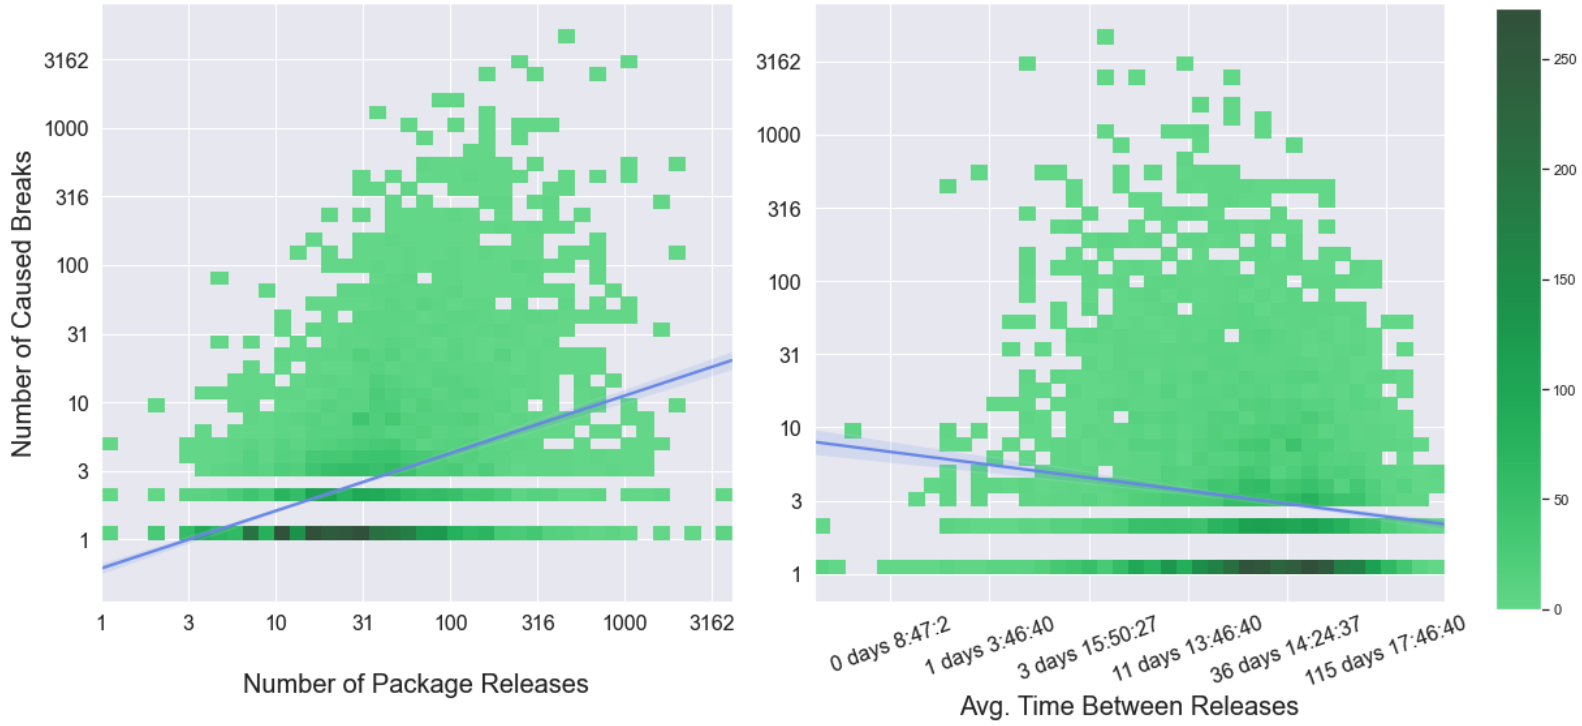
\includegraphics[width=15cm]{images/breakages_to_package_releases_and_frequency_manual.png}
    \caption{Distribution of number of cause breakages and total package releases (left) and release frequency (right)}
    \label{fig:dist_breaks_to_package_release_total_and_freq}
\end{figure*}
\newline
\par
\fbox{%
    \parbox{8cm}{%
        While the majority of clients will accept minor updates, most breakages are caused by patch updates. Packages with higher total and more frequent releases tend to cause more breakages.
    }%
}